\chapter{Results}
This chapter should encompass your data analysis and findings. Additionally, include relevant tables, figures, and citations to support your results and interpretations. Here is a suggested list of topics to discuss:

  \section{Experiments and Tests}
  Describe the experiments conducted to assess the performance of your project. Explain how you collected and processed the data.



\section{Experimentos y Pruebas}

\section{Comparación de Interfaces}
Durante el desarrollo de este proyecto, se llevaron a cabo diversos experimentos con el fin de optimizar el rendimiento de un simulador cuántico de moléculas. En este contexto, la elección de la interfaz para el cálculo de las funciones de coste resulta determinante, pues estas funciones deben optimizarse para obtener el estado y la geometría óptimos de cada molécula. Usualmente, la interfaz \textit{JAX} es la más utilizada gracias a su capacidad de aceleración por GPU, lo que suele proporcionar mayor eficiencia y rapidez en la búsqueda del mínimo de la función de coste.

No obstante, al comparar dos implementaciones idénticas —variando únicamente la interfaz de cálculo—, observamos un resultado sorprendente: la interfaz basada en \textit{JAX}, que se ejecutaba sobre GPU, era más lenta que la interfaz basada en \textit{autograd}, que corría en CPU. Para confirmar que no se trataba de un error en el código, repetimos los experimentos en diferentes máquinas, obteniendo el mismo resultado. Por este motivo, decidimos continuar con la interfaz \textit{autograd}, debido a su mayor rapidez en nuestra implementación específica.

\subsection{Optimización y Registro de Tiempos}
Para constatar las diferencias de rendimiento entre ambas interfaces, se ejecutó la misma optimización variando únicamente la interfaz. Durante estas simulaciones, se registraron los tiempos de ejecución de las distintas funciones del código, cuyos valores se muestran en la Tabla~\ref{tab:comparison_gd}.

\begin{table}[H]
  \centering
  \scriptsize
  \resizebox{\textwidth}{!}{%
  \begin{tabular}{lcccccc}
  \toprule
  \textbf{Function} & 
  \textbf{[\texttt{Li}, \texttt{H}] \_autograd\_GD} & 
  \textbf{[\texttt{Li}, \texttt{H}] \_jax\_GD} & 
  \textbf{[\texttt{O}, \texttt{H}, \texttt{H}] \_autograd\_GD} & 
  \textbf{[\texttt{O}, \texttt{H}, \texttt{H}] \_jax\_GD} & 
  \textbf{[\texttt{H}, \texttt{H}] \_autograd\_GD} & 
  \textbf{[\texttt{H}, \texttt{H}] \_jax\_GD} \\
  \midrule
  Iteration 1  & 1246.7627 & 6251.3362 & 6942.21696 & 39003.89009 & 14.6908 & 40.5485 \\
  Iteration 2  & 1244.0321 & 6284.9812 & 6935.09353 & 40652.7751  & 14.7824 & 36.2979 \\
  Iteration 3  & 1247.4399 & 6348.2470 & 6920.68571 & 40386.29868 & 14.9931 & 38.6236 \\
  Iteration 4  & 1245.7256 & 6351.6437 & 6942.60873 & 40128.31419 & 15.0694 & 39.1362 \\
  Iteration 5  & 1244.8591 & 6349.5099 & 6965.70663 & 40657.74473 & 15.1512 & 40.6186 \\
  \midrule
  \textbf{Total Time} & 6228.8195 & 31585.7475 & 34706.3116 & 200829.0866 & 74.6870 & 195.2551 \\
  \textbf{build\_hamiltonian} & 29.1349   & 30.3407  & 78.4744   & 85.7532   & 0.4934   & 0.5329  \\
  \textbf{compute\_operator\_gradients} & 1533.0319 & 17497.4381 & 12563.3726 & 113792.7167 & 0.6313   & 11.9006 \\
  \textbf{update\_parameters\_and\_coordinates} & 4666.6385 & 14056.6795 & 22064.4153 & 86946.6021 & 73.5594 & 182.5271 \\
  \bottomrule
  \end{tabular}%
  }
  \caption{Tiempos de ejecución para distintas moléculas e interfaces, utilizando \textit{Gradient Descent}.}
  \label{tab:comparison_gd}
\end{table}

En la Figura~\ref{fig:time_iterations}, se muestra cómo evoluciona el tiempo de ejecución a lo largo de las iteraciones para cada molécula y tipo de interfaz. Es evidente que, en todos los casos, la interfaz basada en \textit{autograd} ofrece menores tiempos de cómputo que la interfaz basada en \textit{JAX}.

\begin{figure}[H]
  \centering
  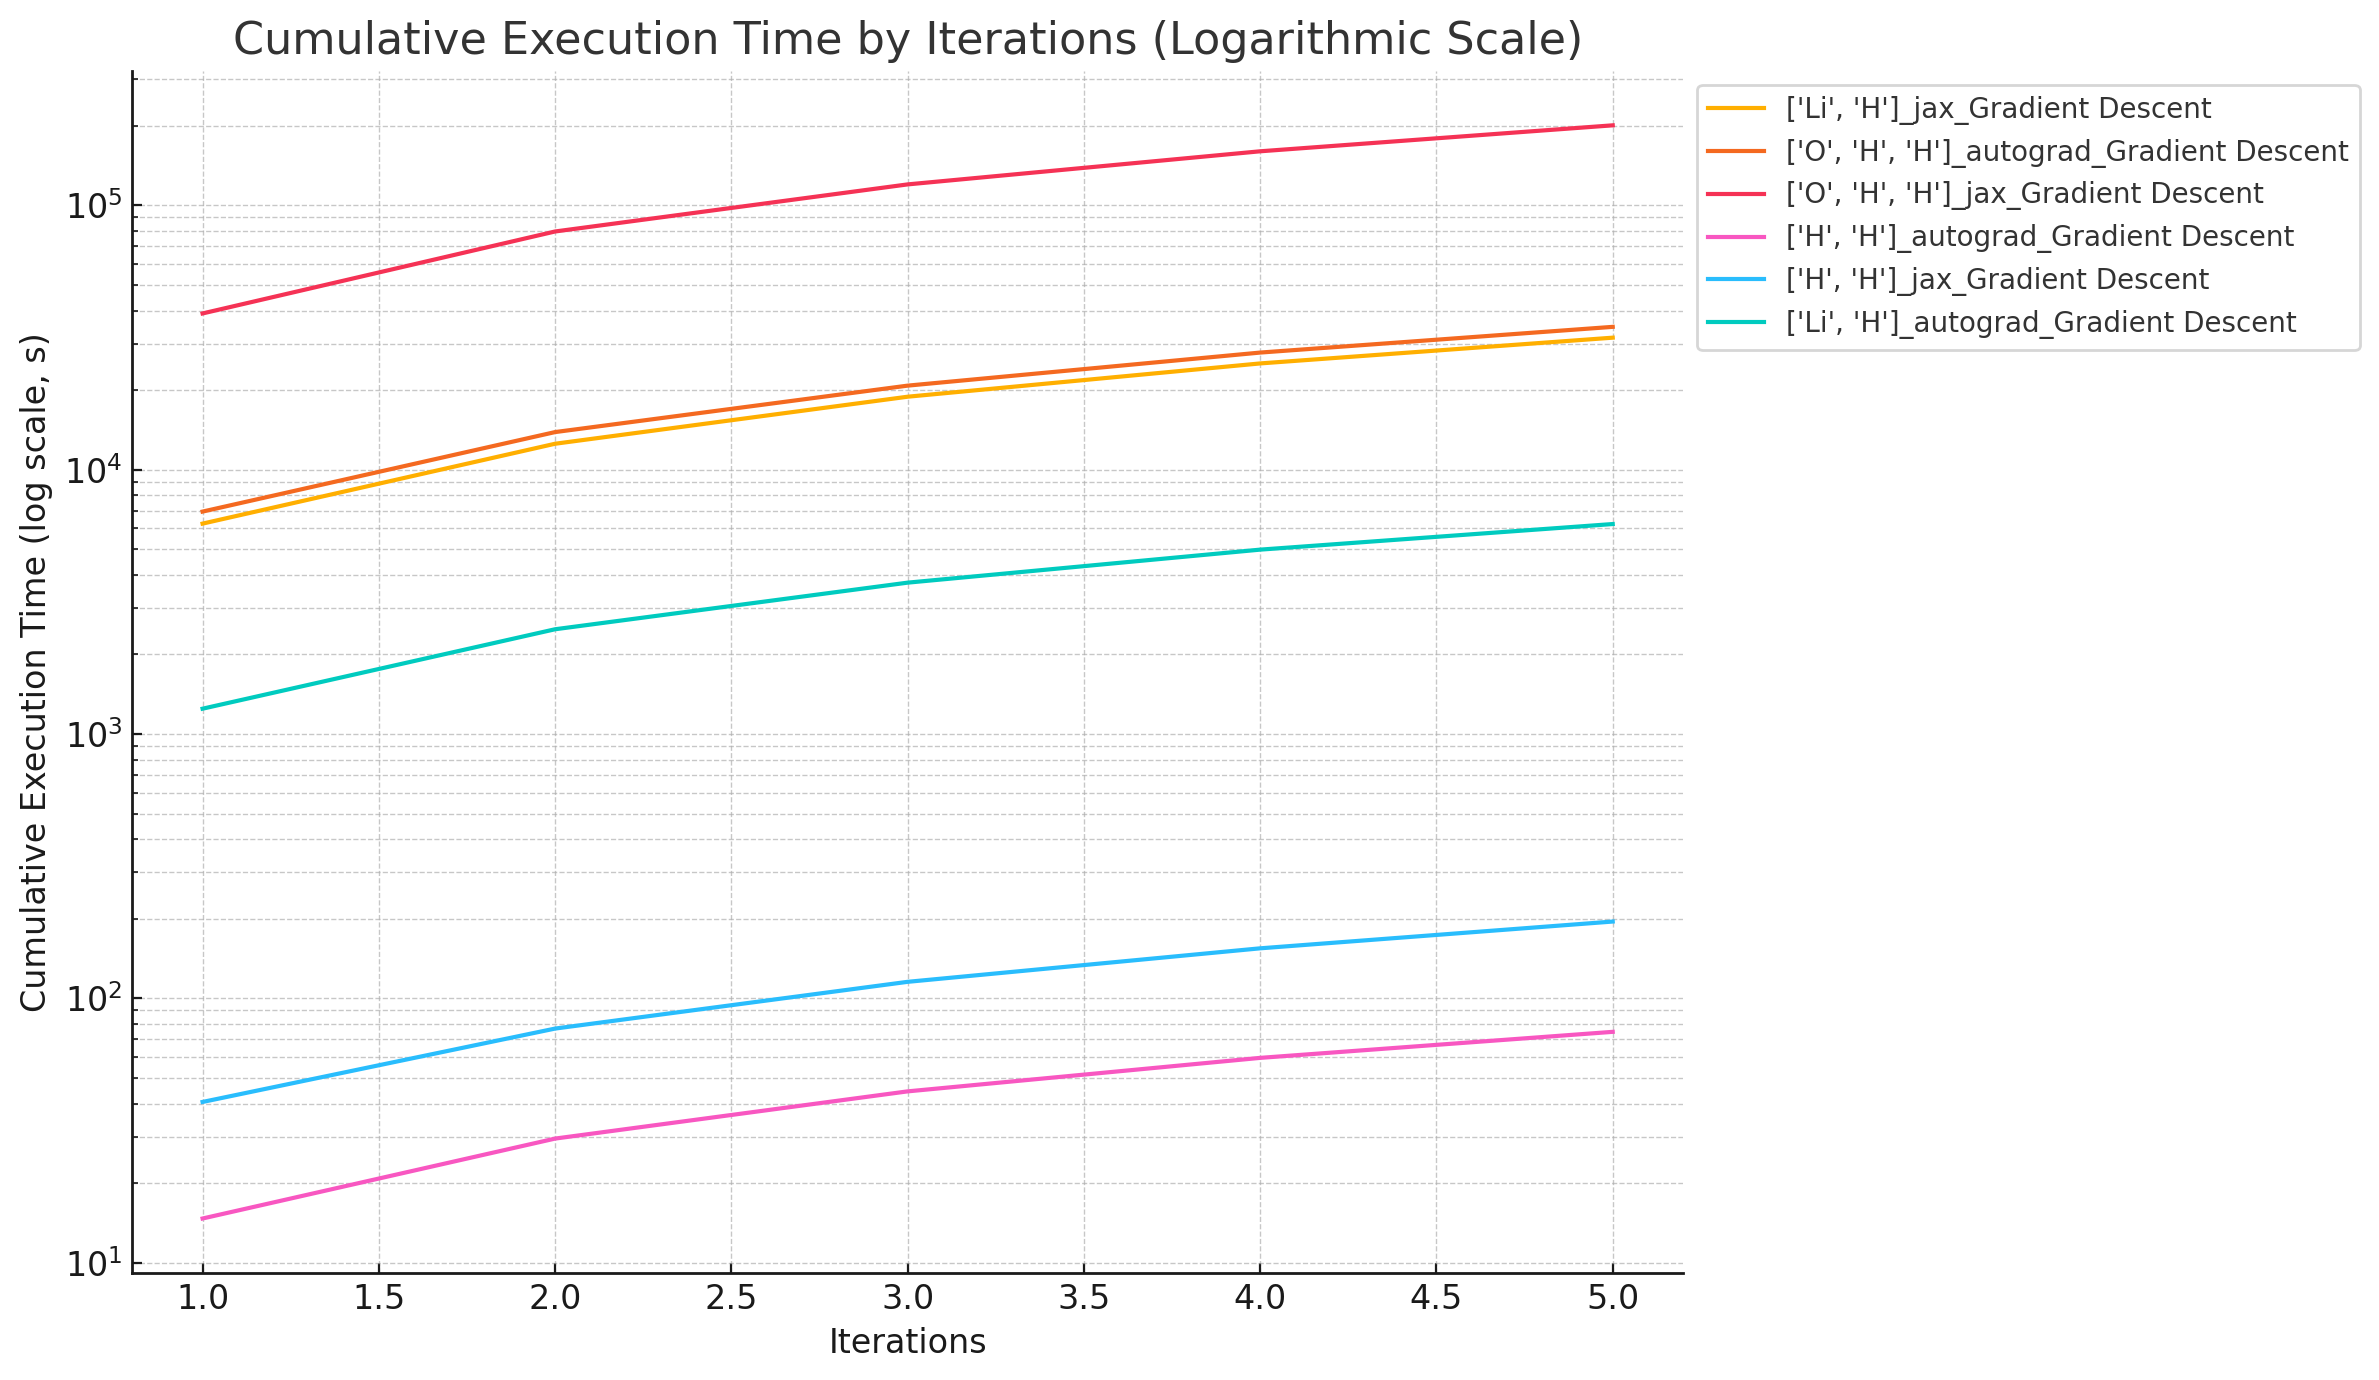
\includegraphics[width=0.8\textwidth]{img/time_iterations.png}
  \caption{Tiempo de ejecución de las distintas moléculas según la iteración en la simulación.}
  \label{fig:time_iterations}
\end{figure}

\subsubsection{Análisis Comparativo de Rendimiento}
Para evaluar de manera más detallada el rendimiento de ambas interfaces, se elaboró una tabla con el porcentaje de incremento en el tiempo de ejecución de \textit{JAX} respecto a \textit{autograd}, tal como se aprecia en la Tabla~\ref{tab:jax_vs_auto}.

\begin{table}[H]
  \centering
  \scriptsize
  \resizebox{\textwidth}{!}{%
  \begin{tabular}{lcccc}
  \toprule
  \textbf{Metric} & 
  \textbf{LiH} & 
  \textbf{H\textsubscript{2}} & 
  \textbf{H\textsubscript{2}O} & 
  \textbf{Mean} \\
  \midrule
  \textbf{Total Time} & 80.28\% & 82.72\% & 61.75\% & 74.92\% \\
  \textbf{build\_hamiltonian} & 3.97\% & 8.49\% & 7.42\% & 6.63\% \\
  \textbf{compute\_operator\_gradients} & 91.24\% & 88.96\% & 94.70\% & 91.63\% \\
  \textbf{update\_parameters\_and\_coordinates} & 66.80\% & 74.62\% & 59.70\% & 67.04\% \\
  \bottomrule
  \end{tabular}%
  }
  \caption{Comparación de tiempos de ejecución entre las interfaces JAX y autograd para diferentes moléculas.}
  \label{tab:jax_vs_auto}
\end{table}

En promedio, se observó que la interfaz \textit{JAX} exhibe un 74.92\% más de tiempo de ejecución total que la interfaz \textit{autograd}. Además, también resulta interesante notar que conforme se incrementa la complejidad de la molécula (mayor número de átomos), el porcentaje de penalización de \textit{JAX} tiende a disminuir. Este comportamiento sugiere que, en problemas de mayor escala, la aceleración por GPU podría llegar a ser más competitiva, aunque no logra superar a \textit{autograd} en esta implementación.

\subsection{Tiempo de Cómputo por Función}
Para un mayor nivel de detalle, se midió también el tiempo de cómputo en cada parte del código, donde se introduce el cambio de interfaz. En la Figura~\ref{fig:time_functions}, se muestran los tiempos de ejecución acumulados en las principales etapas del algoritmo.

\begin{figure}[H]
  \centering
  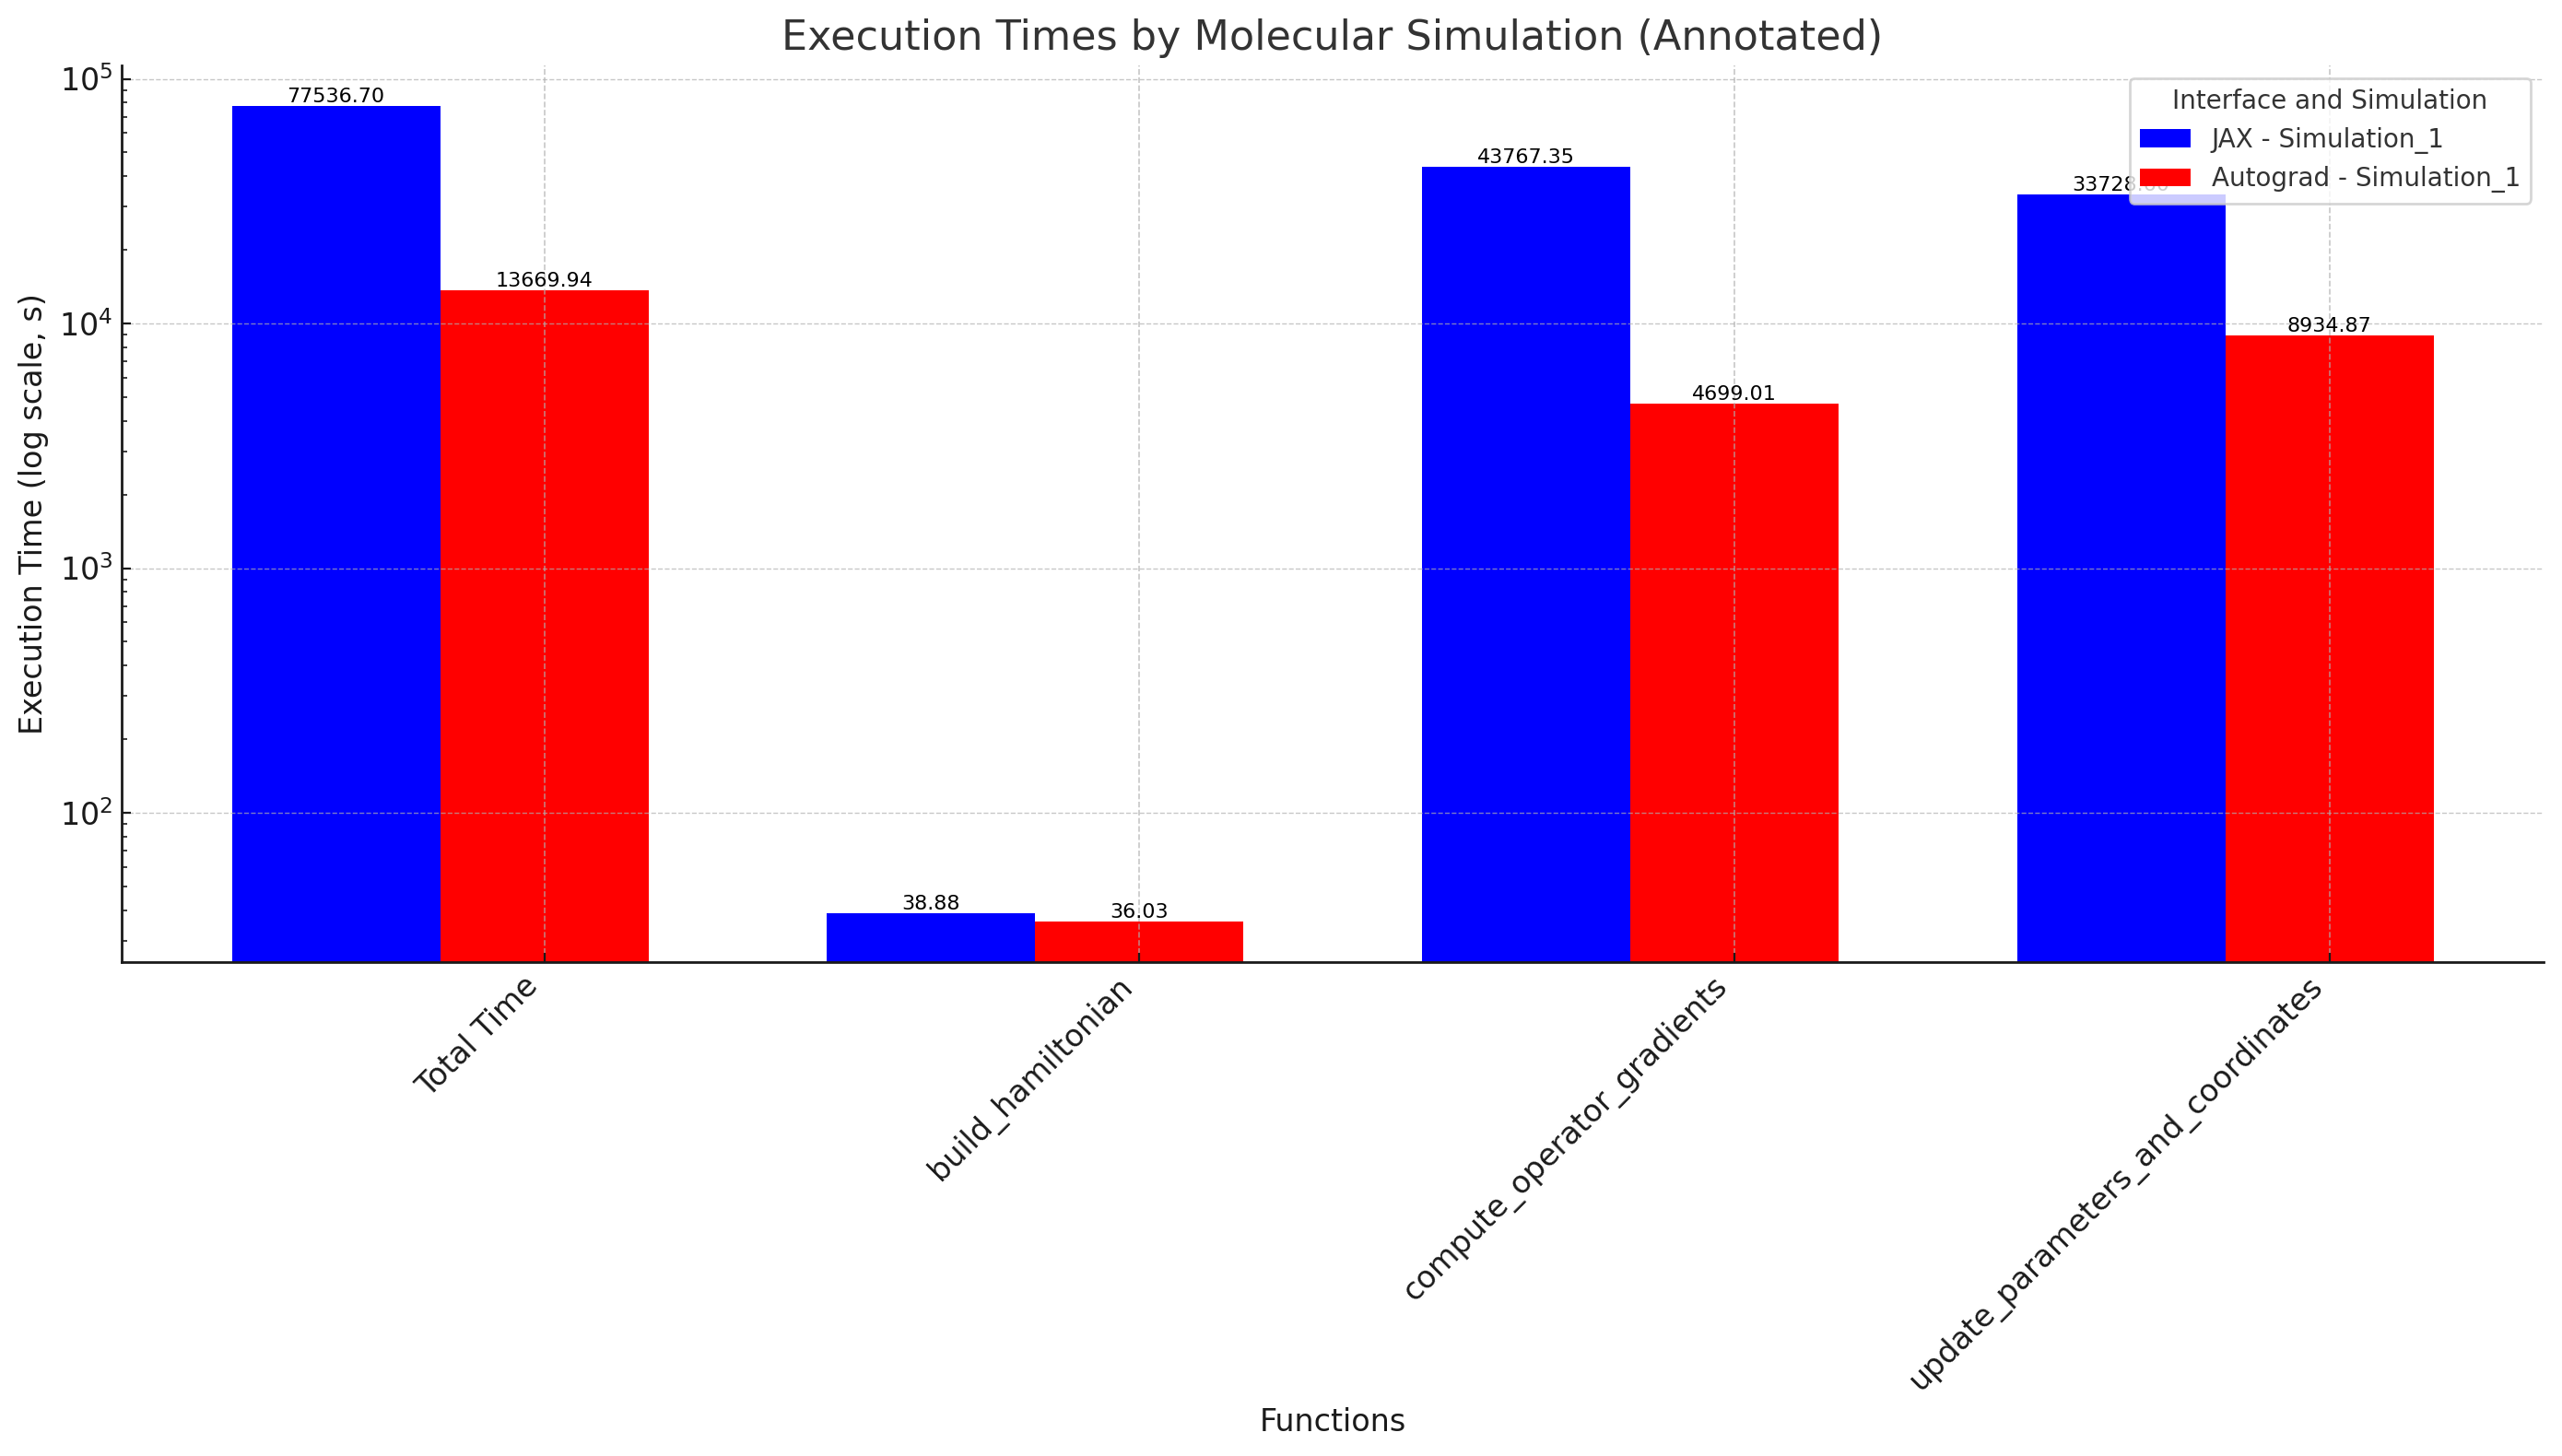
\includegraphics[width=0.8\textwidth]{img/time_functions.png}
  \caption{Tiempo de ejecución en distintas partes del código.}
  \label{fig:time_functions}
\end{figure}

El mismo patrón se mantiene en todas las funciones: la interfaz \textit{JAX} registra mayores tiempos de ejecución que \textit{autograd}. En particular, se observa que la parte de cómputo de gradientes \texttt{compute\_operator\_gradients} incrementa su tiempo de ejecución en un 91.68\% al emplear \textit{JAX}. Esta diferencia se atribuye, en gran medida, al \textit{overhead} causado por la transferencia de datos entre la CPU y la GPU, especialmente cuando \textit{PennyLane} no ofrece soporte completo para generar el Hamiltoniano de la molécula directamente en la GPU.

Por otro lado, la función \texttt{update\_parameters\_and\_coordinates}, encargada de realizar el paso de optimización de la geometría molecular y de los parámetros, también muestra un incremento del 67.04\% al utilizar \textit{JAX}. A pesar de ello, cabe resaltar que, a medida que el problema crece en complejidad, la interfaz \textit{JAX} gana cierta eficiencia relativa en el cálculo de gradientes; sin embargo, el tiempo que se ahorra por la aceleración en GPU se ve contrarrestado por la continua transferencia de datos entre CPU y GPU a lo largo de las iteraciones.

\subsection{Conclusiones}
En base a los resultados obtenidos, la interfaz \textit{autograd} demostró un rendimiento superior en términos de velocidad para nuestra implementación del simulador cuántico molecular. Aunque la GPU suele resultar ventajosa en problemas de mayor escala, el \textit{overhead} de transferencia de datos y la falta de soporte completo en la generación del Hamiltoniano dentro de la GPU redujeron la eficiencia de \textit{JAX}. Por esta razón, finalmente se optó por utilizar la interfaz \textit{autograd} para la implementación definitiva del simulador cuántico de moléculas.

\section{Comparación del Ansatz}
Uno de las modificaciones mas importante y que mas han afectado a nuestro codigo y al funcionamiento de nuestro codigo ha sido la elección del Ansatz. Nuestra propuesta ha sido implementar el UCSSD, un ansatz tipicamente utilizado para este tipo de simulaciones, ya que consigue incrementar el rendimiento de la simulación haciendo que tenga un mayor rendimiento. Ya se a probado la eficacia de este tipo de ansatz y como puede mejorar el rendimiento de las simulaciaciones, consiguiendo circuitos cuanticos mas optimos sin necesidad de crear un ansatz especifico para la molecula a simular. Es un hecho que para cada configuración de optimizadores y para cada simulacion de molecula diferente, existe un circuito quantico optimo que obtiene la mejor performace, pero como nuestro objetivo es poder conseguir un programa que simule con la mayor perfomance distintas moleculas observaremos como la mejor opción es el UCCSD. Para tener una idea de como mejora el rendimiento de nuestra simulación, hemos generado un ansatz con distintos niveles de profundidad y hemos comparado su rendimiento con el rendimiento de un ansatz UCSSD. Hemos simulado distintas configuraciones de ansatz calasicos y en todos los casos, el ansatz UCSSD ha sido el que ha obtenido un mejor rendimiento, se podria probar con ansatz mas complejos y especificos para cada molecula, pero dificilmente encontrariamos otro tipo de ansatz que consia mejorar el rendimiento del UCSSD.

A continuación se muestra una simulación con distintas profundidades de ansatz y distinto numero de iteraciones obtenidas directamente de la simulación.

\begin{figure}[H]
  \centering
  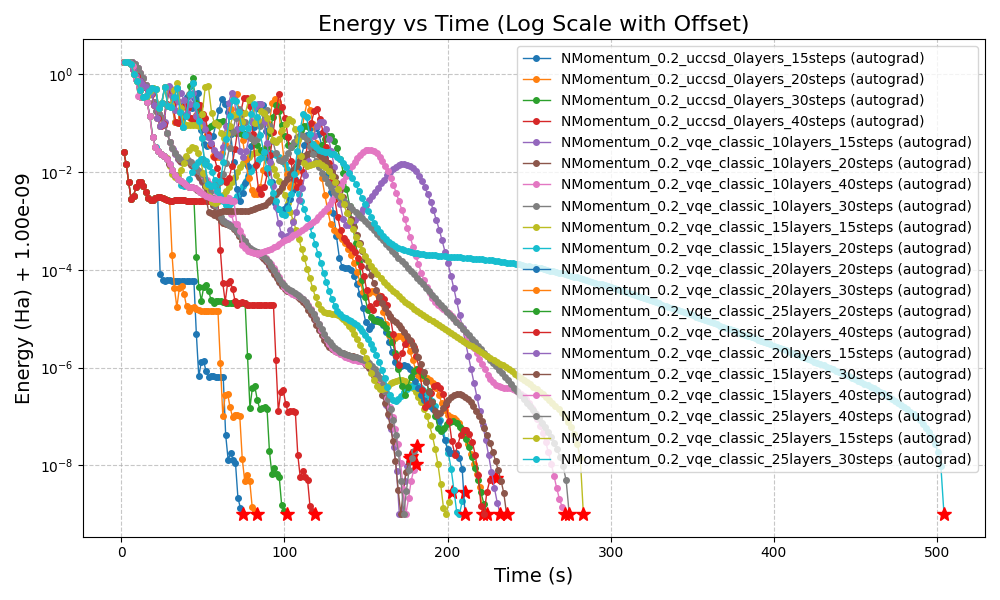
\includegraphics[width=0.8\textwidth]{data/Anzatz/results_ansatz_lyers_dif_iterations/energy_vs_time_log_offset.png}
  \caption{Energy vs Time for different ansatz and iterations.}
  \label{fig:ansatz_layers_iterations}
\end{figure}

Se observa como el ansatz UCSSD es el que mejor rendimiento obtiene en todas las simulaciones independientemente del numero de optimizaciones que se realizen para cada iteración. Para mayor claridad de los resultados, se ha realizado una simulación unicamente con un unico numero de optimizaciones por iteración y se ha comparado el rendimiento de los distintos ansatz, obteniendo una vision mas clara de como le UCCSD es el que mejor rendimiento obtiene.
\begin{figure}[H]
  \centering
  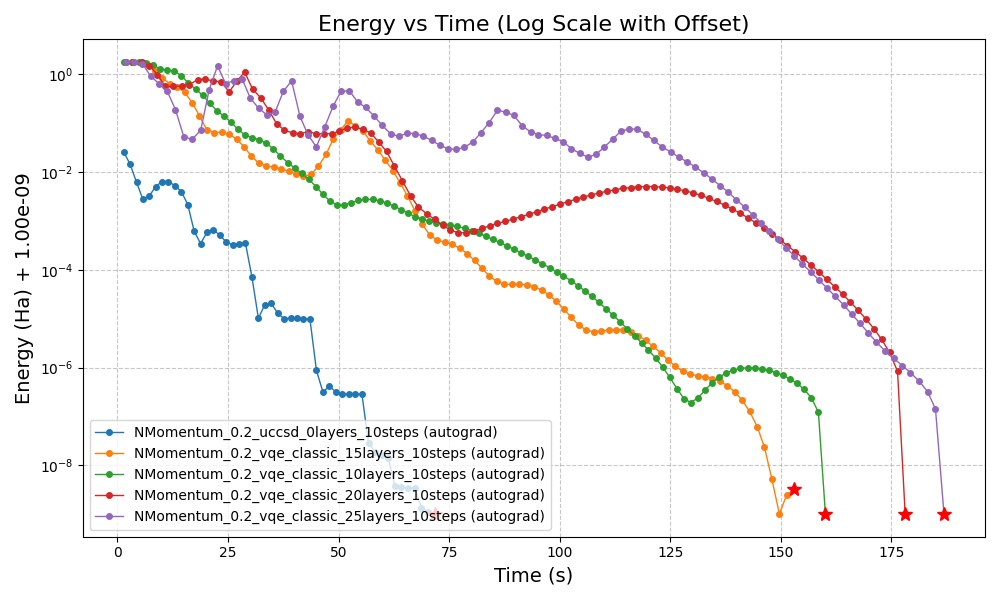
\includegraphics[width=0.8\textwidth]{data/Anzatz/results_ansatz_lyers/energy_vs_time_log_offset.png}
  \caption{Energy vs Time for different ansatz.}
  \label{fig:ansatz_layers}
\end{figure}

Finalmente para corroborar que el ansatz UCSSD es el que mejor rendimiento obtiene, se ha realizado una simulación con otra molecula distinta y se ha comparado el rendimiento de los distintos ansatz. En la siguiente imagen se puede observar como el ansatz UCSSD es el que mejor rendimiento obtiene en todas las simulaciones.



%Hacer simulación para ver cual es la mejor profundidad para el ansatz

%Añadir imagen de la evolución de la energia en función de las iteraciones para distintos ansatz
Como se puede 
\section{Optimizador}

Una vez seleccionado el Ansatz, se procedió a elegir y configurar el optimizador. Para ello, se realizaron simulaciones preliminares con el fin de identificar la mejor configuración.

\subsection{Selección del Optimizador}
Para determinar el optimizador más eficaz en distintas moléculas, se diseñó un conjunto de simulaciones donde se analizó la evolución de la energía en función de las iteraciones. Con este fin, desarrollamos un procedimiento que permitiera ejecutar las mismas moléculas con diversos optimizadores, cada uno abarcando un rango de valores de \emph{step size}. Así, fue posible seleccionar el \emph{step size} más adecuado para cada caso.

En una primera fase, que llegó a ejecutar 42 procesos en paralelo, se observó para cada optimizador y molécula el \emph{step size} que ofrecía el mejor desempeño. Posteriormente, se repitió la simulación empleando únicamente esos \emph{step size} óptimos. Los resultados se muestran a continuación.

\begin{figure}[H]
  \centering
  % Primera imagen
  \begin{subfigure}{0.32\textwidth}
    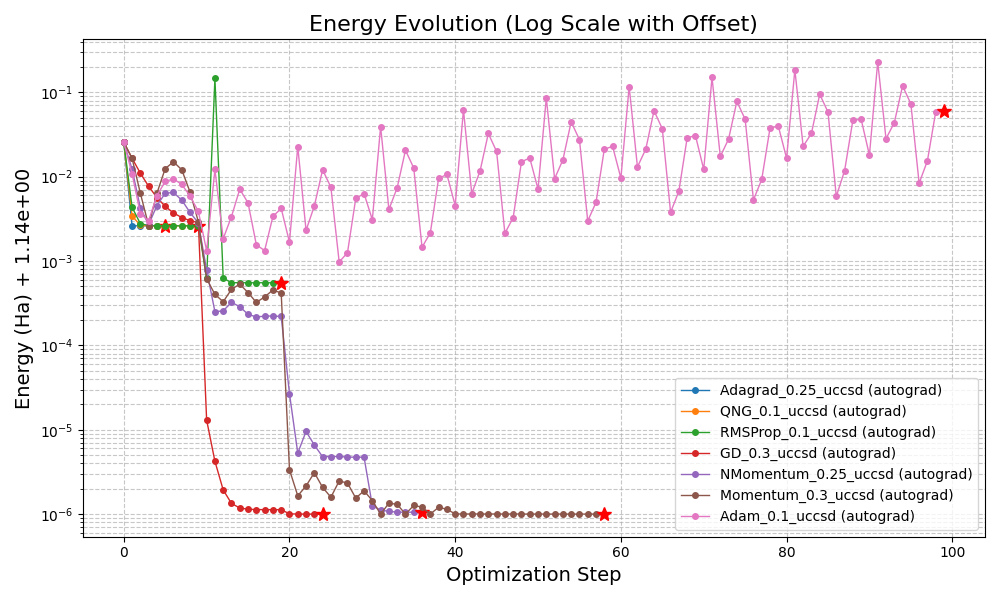
\includegraphics[width=\textwidth]{data/Optimizadores/final_results_H2/energy_evolution_log_offset.png}
    \caption{H2 simulation.}
    \label{fig:subimage1}
  \end{subfigure}
  % Segunda imagen
  \begin{subfigure}{0.32\textwidth}
    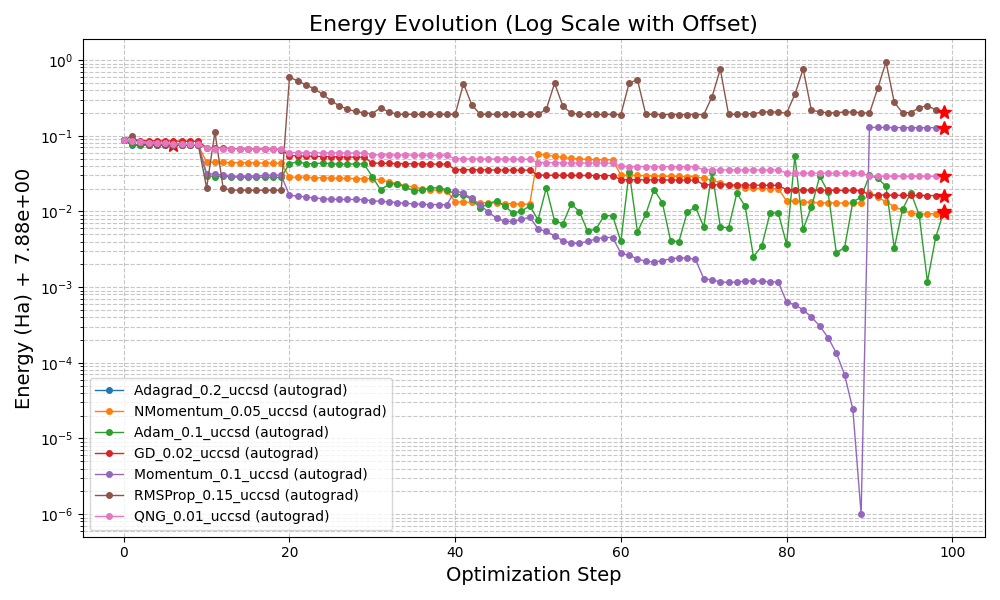
\includegraphics[width=\textwidth]{data/Optimizadores/final_results_LiH/energy_evolution_log_offset.png}
    \caption{LiH simulation.}
    \label{fig:subimage2}
  \end{subfigure}
  % Tercera imagen
  \begin{subfigure}{0.32\textwidth}
    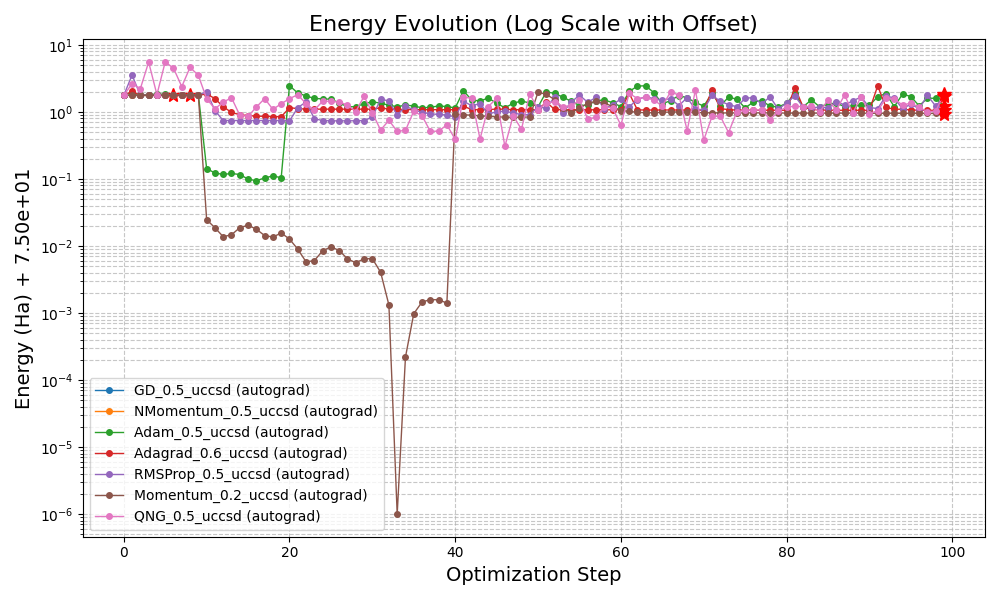
\includegraphics[width=\textwidth]{data/Optimizadores/final_results_H20/energy_evolution_log_offset.png}
    \caption{H2O simulation.}
    \label{fig:subimage3}
  \end{subfigure}
  \caption{Selección óptima de \emph{step size} para cada optimizador y molécula.}
  \label{fig:three_images}
\end{figure}

Para profundizar en el rendimiento de los distintos optimizadores, a continuación se muestran las tablas con la energía final, el tiempo total de optimización y el número de iteraciones necesarias para converger en cada molécula.

\subsubsection{Molécula \(\mathrm{H_2O}\)}

\begin{table}[H]
\centering
\caption{Energía final y tiempo de optimización para \(\mathrm{H_2O}\) (sin usar FCI).}
\begin{tabular}{lccc}
\toprule
\textbf{Optimizador} & \textbf{Energía Final (Ha)} & \textbf{Tiempo Total (s)} & \textbf{Iteraciones}\\
\midrule
Adam (0.5)       & -73.75990609 & 28454.49 & 10 \\
Adagrad (0.6)    & -73.93046296 & 28891.08 & 10 \\
NMomentum (0.5)  & -73.22152796 & 7497.83  &  1 \\
Momentum (0.2)   & \textbf{-74.03997489} & 68420.47 & 10 \\
RMSProp (0.5)    & -73.28585876 & 65470.02 & 10 \\
GD (0.5)         & -73.22152796 & \textbf{6486.79}  &  1 \\
QNG (0.5)        & -73.13971041 & 70716.22 & 10 \\
\bottomrule
\end{tabular}
\end{table}

En esta molécula, la energía más \emph{negativa} la aporta \textbf{Momentum (0.2)}, con \(-74.03997489\)\,Ha, pero a costa de un tiempo muy elevado (68420.47\,s). Por otro lado, \textbf{GD (0.5)} requiere sólo 6486.79\,s, aunque su valor de energía \((-73.22152796)\,\mathrm{Ha}\) es algo menos negativo.

\subsubsection{Molécula \(\mathrm{H_2}\)}

\begin{table}[h!]
\centering
\caption{Energía final y tiempo de optimización para \(\mathrm{H_2}\).}
\begin{tabular}{lccc}
\toprule
\textbf{Optimizador} & \textbf{Energía Final (Ha)} & \textbf{Tiempo Total (s)} & \textbf{Iteraciones}\\
\midrule
Adam (0.1)       & -1.07655292  & 173.30  & 10 \\
Adagrad (0.25)   & -1.13469066  & 10.19   &  1 \\
NMomentum (0.25) & -1.13730600  & 62.84   &  4 \\
Momentum (0.3)   & \textbf{-1.13730605} & 100.43  &  6 \\
RMSProp (0.1)    & -1.13675411  & 33.14   &  2 \\
GD (0.3)         & \textbf{-1.13730605} & 41.77   &  3 \\
QNG (0.1)        & -1.13469066  & 18.40   &  1 \\
\bottomrule
\end{tabular}
\end{table}

En este caso, los valores más negativos (\(-1.13730605\)\,Ha) corresponden tanto a \textbf{Momentum (0.3)} como a \textbf{GD (0.3)}. Si se busca rapidez, \textbf{GD (0.3)} sólo requiere 41.77\,s, siendo una opción muy competitiva.

\subsubsection{Molécula \(\mathrm{LiH}\)}

\begin{table}[H]
\centering
\caption{Energía final y tiempo de optimización para \(\mathrm{LiH}\).}
\begin{tabular}{lccc}
\toprule
\textbf{Optimizador} & \textbf{Energía Final (Ha)} & \textbf{Tiempo Total (s)} & \textbf{Iteraciones}\\
\midrule
Adam (0.1)       & -7.87024707 & 13444.57 & 10 \\
Adagrad (0.2)    & -7.80548501 & 977.86   &  1 \\
NMomentum (0.05) & \textbf{-7.87085783} & 13442.59 & 10 \\
Momentum (0.1)   & -7.75267240 & 13566.98 & 10 \\
RMSProp (0.15)   & -7.67650000 & 13671.22 & 10 \\
GD (0.02)        & -7.86422129 & 13449.49 & 10 \\
QNG (0.01)       & -7.85120449 & 13776.00 & 10 \\
\bottomrule
\end{tabular}
\end{table}

Aquí, el valor más bajo \((-7.87085783)\,\mathrm{Ha}\) se logra con \textbf{NMomentum (0.05)}. Tanto NMomentum (0.05) como Adam (0.1) superan \(-7.870\)\,Ha con tiempos muy similares (ambos rondan los 13400\,s). Por su parte, \textbf{Momentum (0.1)} resulta más lento y menos efectivo en términos de energía.

En síntesis, \emph{no existe un optimizador universalmente óptimo}. La elección depende de la molécula, del coste computacional aceptable y de la meta en términos de energía final. \textbf{Momentum} suele alcanzar los valores más bajos, aunque a veces con altos requerimientos de tiempo. \textbf{GD}, por otro lado, converge con rapidez y ofrece resultados cercanos a los mínimos más negativos en varias de las pruebas. Despues de revisar los resultados obtenidos, nos decantamos por escoger el optimizador Momentum, ya que es el que mejor convergencia obtiene sin necesidad de añadir mucho tiempo en computo.  


\subsection{Selección del Step Size}
Una vez seleccionado el optimizador, se procedió a la selección del step size. Para ello, se tubo en cuenta el mejor humbral de step size obtenido en la selección del optimizador i volvimos a hacer la simulación con distintos step size con valor cercano al optimo. A continuación se muestra la evolución de la energia en función de las iteraciones para distintos step size para cada molecula.



%Añadir imagen de la evolución de la energia en función del step size

Como se puede observar en las tres imagenes, el rango de step size donde mejor funciona el optimizador es entre 0.1 y 0.3. Pasa algo curioso con la molecula H2, y es que el optimizador funciona mejor con un step size de 0.4, un valor relativamente alto. Esto se debe a que justamente, con este valor, el optimizador, por casualidad, consigue llegar a la condición de convergencia que hemos definido, %Explicar la condición de convergencia del codigo.

Aun asi, para observar mas concretamente, el valor de step size que mejor se adaptaba con nuestras simulaciones, decidimos volver a generar las simulaciones de las distintas moleculas con distintos step size, y observar la evolución de la energia en función de las iteraciones. Estos son los resultados.

%Añadir imagen de la evolución de la energia en función de las iteraciones para distintos step size

De igual manera que antes, se observa que dependiendo de la simulación, el valor de step size idoneo va variando segun el 


\subsection{Numero de Iteraciones}

Finalmente, una de los procesos donde mas tiempo se consume en la simulación es en la actualización de parametros y de las coordenadas, en esta ultima prueba lo que queremos conseguir es poder optimizar el numero de iteraciones que se actualizan los parametros y las coordenadas antes de volver a calcular el Hamiltoniano. Para ello, hemos generado una serie de simulaciones con distintos numeros de iteraciones, y hemos observado la evolución de la energia en función de las iteraciones. La configuarción de los optimizadores, han sido con los valores optimos que hemos obtenido despues de haber hecho todas las pruebas, como se podra observar en las imagenes 